% Provenance (never printed): see sources/outline_sources.md (Year 3:
% Glen's flow law; mass balance; ice sheets and ice shelves; sea ice;
% permafrost; the cryosphere's contribution to sea level).
% Brief: sources/book5/BRIEFS.md, ch. 24. Curves from figdata/bachelor-3/
% ice_flow.py (Glen slab, the plastic profile against the ETOPO1 Greenland
% transect, the Arkel ice cap) and sea_ice.py (NSIDC March and September
% extents, Stefan's law). Exercise and problem values in the Book 5 scratch
% calculator calc/ch24.py. The Arkel ice cap and the glaciers of the
% exercises are invented.
\chapter{Glaciologia}\label{ch:b3:glaciology}

Atravessa-se a Groenlândia de O para L ao longo do paralelo \ang{72.5}N. O gelo
começa a poucas dezenas de quilômetros para o interior, sobe de forma íngreme e, depois, cada vez mais suavemente,
até um cume amplo, com \qty{3229}{m} de altura, e desce novamente até as montanhas da
costa leste. Representada em gráfico, a superfície se aproxima de uma parábola deitada de lado,
com o vértice na margem. Este capítulo mostra de onde vem essa forma:
de um material que se deforma por fluência cada vez mais depressa à medida que é mais solicitado,
de modo que se comporta quase como se não suportasse mais do que certa tensão.
Em seguida, acompanha-se o gelo desde a neve que o alimenta até o mar que o
recebe.
% ledger: data:b5-etopo-greenland

\begin{recall}
Geleiras, mantos de gelo, plataformas de gelo, icebergs, gelo marinho, permafrost e as
eras glaciais estão nos livros escolares. As \omterm{def:b3:deformation-mechanisms:flow-law}{leis de fluxo} e a \omterm{def:b3:deformation-mechanisms:creep}{fluência por deslocações}
estão no Capítulo~\ref{ch:b3:deformation-mechanisms}; a \omterm{def:b3:gravity-geodesy:satgrav}{gravimetria por satélite} e o
balanço de massa do manto de gelo que ela mede no Capítulo~\ref{ch:b3:gravity-geodesy};
os testemunhos de gelo e seus isótopos de oxigênio no Capítulo~\ref{ch:b3:stable-isotopes}.
O balanço do nível do mar, a retroalimentação gelo--albedo e a elevação termostérica do
nível do mar estão no volume do segundo ano, no capítulo sobre mudança climática
antropogênica. O calor latente e a condução de calor estão nos livros de física.
\end{recall}

\section{O gelo como material}\label{sec:b3:glaciology:material}

O gelo de geleira é uma rocha, uma massa de cristais de gelo entrelaçados, e se deforma
próximo do seu ponto de fusão. Sob uma tensão, ele se deforma por fluência pelo
movimento de deslocações em seus cristais, como as rochas do
Capítulo~\ref{ch:b3:deformation-mechanisms}, e sua \omterm{def:b3:deformation-mechanisms:flow-law}{lei de fluxo} tem a mesma
forma: uma potência da tensão multiplicada por um fator de Arrhenius.

\begin{theorem}[Lei de fluxo de Glen]\label{thm:b3:glaciology:glen}
No gelo de geleira isotrópico, o tensor da taxa de deformação é proporcional à
tensão desviatória,
\[
\dot\varepsilon_{ij} = A(T)\,\tau_e^{\,n-1}\,\tau'_{ij}, \qquad
\tau_e^2 = \tfrac12\,\tau'_{ij}\tau'_{ij},
\]
com $n = 3$ e um \omterm{def:b3:glaciology:glen}{fator de taxa} $A(T)$ que cresce com a temperatura. Em
cisalhamento simples, com $\tau_{xz}$ como a única tensão desviatória não nula,
$\dot\varepsilon_{xz} = A\tau_{xz}^{\,n}$.
\end{theorem}
\index{Lei de fluxo de Glen}

\begin{proof}
A própria lei é empírica: uma lei de potência ajustada a experimentos de fluência e
à deformação de geleiras, com o coeficiente e o expoente ajustados
em conjunto. Em cisalhamento simples $\tau'_{xz} = \tau'_{zx} = \tau_{xz}$ e as
demais componentes se anulam, logo $\tau_e^2 = \tfrac12(\tau_{xz}^2 +
\tau_{zx}^2) = \tau_{xz}^2$, e $\dot\varepsilon_{xz} = A\tau_{xz}^{\,n-1}
\tau_{xz}$.
\end{proof}
% ledger: pism:rheology

Com $n = 3$, o gelo é um fluido fortemente não linear: dobrar a tensão faz com que
ele se deforme oito vezes mais depressa. Sua viscosidade efetiva, $1/(2A\tau_e^{\,2})$,
não é uma propriedade só do gelo, mas diminui à medida que a tensão aumenta.

\begin{definition}[Fator de taxa (gelo)]\label{def:b3:glaciology:glen}
O \emph{fator de taxa}\index{fator de taxa (gelo)} $A(T)$ da lei de Glen, também
chamado de fluidez do gelo, escreve-se $A = A_0\exp(-Q/RT)$, com uma
energia de ativação $Q$. Um ajuste amplamente usado (Paterson e Budd) adota $A_0 =
\qty{3.61e-13}{s^{-1}.Pa^{-3}}$ e $Q = \qty{60}{kJ/mol}$ abaixo de
\qty{-10}{\celsius}, e $A_0 = \qty{1.73e3}{s^{-1}.Pa^{-3}}$ e $Q =
\qty{139}{kJ/mol}$ acima dela, mais próximo do ponto de fusão, onde o gelo
amolece mais depressa com a temperatura.
\end{definition}
% ledger: pism:rheology, codata:R

\begin{center}
\begin{tabular}{lccc}
\hline
temperatura & \qty{-25}{\celsius} & \qty{-10}{\celsius} & \qty{0}{\celsius}\\
$A$ (\unit{Pa^{-3}.yr^{-1}}) & \num{2.7e-18} & \num{1.4e-17} & \num{1.4e-16}\\
\hline
\end{tabular}
\end{center}

O gelo no seu ponto de fusão flui cerca de cinquenta vezes mais depressa do que a
\qty{-25}{\celsius} sob a mesma tensão. As tensões nas geleiras são da ordem de
um bar, \qty{e5}{Pa}.
% ledger: pism:rheology

Uma geleira se move de duas maneiras. Seu gelo se deforma por fluência, em toda parte; e
onde o leito está no ponto de fusão, ela também pode deslizar.

\begin{definition}[Deslizamento basal]\label{def:b3:glaciology:sliding}
O \emph{deslizamento basal}\index{deslizamento basal} é o movimento de uma geleira sobre
seu leito, sobre uma película fina de água ou uma camada de sedimento mole e úmido. Ele
requer um leito no ponto de fusão; uma geleira congelada ao leito se move apenas
pela fluência do seu gelo.
\end{definition}
% ledger: nsidc:glacier-flow

\section{Fluxo glacial}\label{sec:b3:glaciology:flow}

\begin{theorem}[Escoamento de uma placa de lados paralelos]\label{thm:b3:glaciology:slab}
Uma placa de gelo de espessura $H$ e densidade $\rho$ repousa sobre um leito de declive
$\alpha$ e desce por ele por cisalhamento simples, deslizando com velocidade $u_b$. A
altura $z$ acima do leito, a tensão de cisalhamento é $\tau = \rho g(H - z)\sin\alpha$,
a velocidade
\[
u(z) = u_b + \frac{2A}{n + 1}(\rho g\sin\alpha)^n\left[H^{n+1} - (H -
z)^{n+1}\right],
\]
e o fluxo por unidade de largura $q = u_bH + \dfrac{2A}{n + 2}(\rho
g\sin\alpha)^nH^{n+2}$. A tensão de cisalhamento basal é $\tau_b = \rho gH\sin\alpha$.
\end{theorem}

\begin{proof}
O gelo acima da altura $z$ tem peso $\rho g(H - z)$ por unidade de área; sua
componente ao longo do declive, $\rho g(H - z)\sin\alpha$, é equilibrada pela
tensão de cisalhamento em sua base, sendo a superfície livre de tensão. Pela lei de Glen,
$\mathrm du/\mathrm dz = 2\dot\varepsilon_{xz} = 2A\tau^n$; integrando a partir
do leito, onde $u = u_b$, obtém-se $u(z)$, e integrando $u$ de 0 a $H$
obtém-se $q$.
\end{proof}

A velocidade muda pouco na parte superior da placa e cresce rapidamente perto do
leito, onde a tensão é maior: com $n = 3$, o cisalhamento concentra-se nas
camadas mais baixas. A velocidade superficial cresce com $H^{n+1} = H^4$ e com o
cubo do declive: uma geleira com o dobro da espessura flui dezesseis vezes mais depressa.

\begin{definition}[Aproximação de gelo raso]\label{def:b3:glaciology:sia}
A \emph{aproximação de gelo raso}\index{aproximação de gelo raso} trata
um manto de gelo cuja espessura é pequena em relação à sua largura como, localmente, uma
placa de lados paralelos: em cada ponto, o gelo se deforma por cisalhamento simples sob
a \emph{tensão motriz} $\tau_d = \rho gH|\nabla s|$, sendo $s$ a elevação da
superfície, e o fluxo segue a fórmula da placa com a espessura local e o
declive superficial local.
\end{definition}

Na \omterm{def:b3:glaciology:sia}{aproximação de gelo raso}, a tensão basal é definida pela forma do
gelo. Como a taxa de deformação cresce com o cubo da tensão, um aumento modesto de
tensão produz um grande aumento de fluxo, que afina o gelo
e reduz novamente a tensão: a tensão permanece dentro de uma faixa estreita,
qualquer que seja o tamanho da massa de gelo. Levando isso ao limite, um material que
não se deforma de modo algum abaixo de uma tensão de escoamento $\tau_0$ e se deforma sem
limite acima dela, e a forma segue.

\begin{proposition}[Perfil de um manto de gelo plástico]\label{prop:b3:glaciology:nye}
Um manto de gelo perfeitamente plástico, com tensão de escoamento $\tau_0$, sobre um
leito horizontal plano tem, à distância $x$ para o interior a partir de sua margem, a altura da superfície
\[
h(x) = \sqrt{\frac{2\tau_0x}{\rho g}} .
\]
\end{proposition}
\index{perfil de um manto de gelo plástico}

\begin{proof}
Em toda parte, a tensão basal é igual à tensão de escoamento: $\rho gh\,\mathrm
dh/\mathrm dx = \tau_0$, sendo o declive pequeno. Então $\mathrm d(h^2)/\mathrm
dx = 2\tau_0/(\rho g)$, e $h = 0$ na margem.
\end{proof}

\begin{omfigure}
\begin{tikzpicture}
\begin{groupplot}[group style={group size=2 by 1, horizontal sep=1.5cm},
  height=0.4\linewidth,
  tick label style={font=\scriptsize}, label style={font=\small}, title style={font=\small}]
\nextgroupplot[width=0.38\linewidth, xlabel={$u/u_s$}, ylabel={altura acima do leito, $z/H$},
  xmin=0, xmax=1.05, ymin=0, ymax=1, title={uma placa},
  legend style={font=\scriptsize, at={(0.03,0.97)}, anchor=north west}]
% computed in figdata/bachelor-3/ice_flow.py
\addplot[omThm, thick] table[x=u3, y=zeta] {figdata/out/bachelor-3-ice_flow-slab.dat};
\addlegendentry{$n = 3$}
\addplot[omDef, thick, densely dashed] table[x=u1, y=zeta] {figdata/out/bachelor-3-ice_flow-slab.dat};
\addlegendentry{$n = 1$}
\addplot[omMeth, thick] table[x=u3b, y=zeta] {figdata/out/bachelor-3-ice_flow-slab.dat};
\addlegendentry{$n = 3$, deslizamento}
\nextgroupplot[width=0.58\linewidth, xlabel={distância de \ang{58}O ao longo de \ang{72.5}N (\unit{km})},
  ylabel={elevação (\unit{m})}, xmin=0, xmax=1270, ymin=-500, ymax=3700,
  title={Groenlândia}, scaled x ticks=false, xticklabel style={/pgf/number format/1000 sep={}},
  scaled y ticks=false, yticklabel style={/pgf/number format/1000 sep={}},
  legend style={font=\scriptsize, at={(0.5,0.03)}, anchor=south}]
\addplot[black, thin] table[x=x, y=h] {figdata/out/bachelor-3-ice_flow-gl.dat};
\addlegendentry{gelo e superfície do terreno}
\addplot[omThm, thick, densely dashed] table[x=x, y=h] {figdata/out/bachelor-3-ice_flow-nye-w.dat};
\addlegendentry{perfis plásticos}
\addplot[omThm, thick, densely dashed, forget plot] table[x=x, y=h] {figdata/out/bachelor-3-ice_flow-nye-e.dat};
\draw[black!40] (axis cs:0,0) -- (axis cs:1270,0);
\node[font=\scriptsize, omThm, align=center] at (axis cs:330,2900) {$\tau_0 = $\\ \qty{72}{kPa}};
\node[font=\scriptsize, omThm, align=center] at (axis cs:1040,2900) {$\tau_0 = $\\ \qty{108}{kPa}};
\end{groupplot}
\end{tikzpicture}

\par\smallskip{\small À esquerda, a velocidade através de uma placa de gelo, escalada pela
velocidade superficial: a lei de Glen ($n = 3$) concentra o cisalhamento perto do leito, enquanto
um fluido linear ($n = 1$) o distribui; com deslizamento, o perfil inteiro é
deslocado. À direita, a superfície da Groenlândia ao longo de \ang{72.5}N (ETOPO1 Ice
Surface, NOAA NCEI), e os perfis plásticos ajustados a seus dois lados, para
alturas acima de \qty{1000}{m} e um leito tomado ao nível do mar. Os ajustes exigem
tensões de escoamento de \qty{72}{kPa} e \qty{108}{kPa}, da ordem do bar
das geleiras reais; eles não capturam as margens íngremes, onde o leito e o derretimento
importam.}\label{fig:b3:glaciology:flow}
\end{omfigure}
% ledger: data:b5-etopo-greenland, pism:rheology

\section{Balanço de massa}\label{sec:b3:glaciology:mass-balance}

Uma geleira é alimentada por neve e perde gelo por derretimento, evaporação e, onde
alcança a água, por desprendimento.
% ledger: nsidc:glacier-zones

\begin{definition}[Balanço de massa; zonas de acumulação e de ablação; linha de equilíbrio]\label{def:b3:glaciology:mass-balance}
O \emph{balanço de massa da geleira}\index{balanço de massa da geleira} é a variação
da massa de uma geleira ao longo de um ano, geralmente expressa em metros de água
equivalente, média sobre sua área. O \emph{balanço de massa
superficial}\index{balanço de massa superficial} é a parcela devida aos processos na
superfície, a queda de neve menos o derretimento, o escoamento superficial e a sublimação; o restante é
perdido por desprendimento e por derretimento na base ou sob o gelo flutuante. A
\emph{zona de acumulação}\index{zona de acumulação} é a parte da
superfície onde o balanço de massa superficial ao longo de um ano é positivo, a
\emph{zona de ablação}\index{zona de ablação} a parte onde ele é negativo,
e a \emph{altitude da linha de equilíbrio}\index{altitude da linha de equilíbrio}
(ELA) é a elevação da linha que as separa, onde ele é zero.
\end{definition}

\begin{omfigure}
\centering
\begin{tikzpicture}[>=stealth, font=\small, x=1cm, y=1cm]
% bed and surface of a valley glacier, long section
\fill[black!12] (0,0) -- (0,4.6) .. controls (2,3.6) and (6,1.4) .. (11,0) -- cycle;
\fill[omSea!45] (0,4.6) .. controls (2,3.6) and (6,1.4) .. (11,0)
  -- (11,0) .. controls (8,1.0) and (4,3.2) .. (0.6,5.4) -- (0,5.6) -- cycle;
\draw[thick, black!70] (0,4.6) .. controls (2,3.6) and (6,1.4) .. (11,0);
\draw[thick, omDef] (0,5.6) -- (0.6,5.4) .. controls (4,3.2) and (8,1.0) .. (11,0);
% equilibrium line
\draw[omThm, densely dashed, thick] (5.0,2.76) -- (5.0,4.6);
\node[omThm, font=\scriptsize, anchor=south] at (5.0,4.6) {linha de equilíbrio (ELA)};
% balance arrows
\foreach \x/\y in {1.2/5.02, 2.4/4.27, 3.6/3.56} {\draw[->, omDef, thick] (\x,\y+0.55) -- (\x,\y+0.05);}
\foreach \x/\y in {6.4/2.02, 7.6/1.42, 8.8/0.86} {\draw[->, omThm, thick] (\x,\y+0.02) -- (\x,\y+0.52);}
\node[omDef, font=\scriptsize, align=center] at (2.4,6.2) {zona de acumulação:\\neve acumulada};
\node[omThm, font=\scriptsize, align=center] at (8.6,2.5) {zona de ablação:\\gelo perdido};
% flow lines, computed inside the ice: buried in the accumulation zone, emerging in the ablation zone
\draw[->, black!60] plot[smooth] coordinates {(1.00,5.14) (1.98,4.28) (2.95,3.54) (3.93,2.93) (4.90,2.43) (5.88,2.00) (6.85,1.62) (7.83,1.24) (8.80,0.86)};
\draw[->, black!60] plot[smooth] coordinates {(2.20,4.39) (2.84,3.89) (3.48,3.43) (4.11,3.02) (4.75,2.67) (5.39,2.36) (6.03,2.08) (6.66,1.82) (7.30,1.56)};
\draw[->, black!60] plot[smooth] coordinates {(3.40,3.67) (3.74,3.44) (4.08,3.21) (4.41,3.00) (4.75,2.81) (5.09,2.63) (5.42,2.47) (5.76,2.32) (6.10,2.17)};
\node[font=\scriptsize, anchor=north east] at (10.9,-0.1) {língua};
\node[font=\scriptsize] at (3.0,1.4) {substrato rochoso};
\end{tikzpicture}

\par\smallskip{\small Perfil longitudinal esquemático de uma geleira de vale em
equilíbrio. Acima da linha de equilíbrio, a neve de cada ano fica soterrada e
é transportada para o interior da geleira; abaixo dela, a superfície perde gelo a cada ano e
é renovada pelo gelo que ascende das profundezas. As linhas de fluxo (cinzas) descem na
\omterm{def:b3:glaciology:mass-balance}{zona de acumulação} e sobem na \omterm{def:b3:glaciology:mass-balance}{zona de ablação}; o fluxo leva o
excedente de uma zona ao déficit da outra.}\label{fig:b3:glaciology:zones}
\end{omfigure}
% ledger: nsidc:glacier-zones, nsidc:glacier-flow

Nos mantos de gelo e nas geleiras de altitude, a neve não se transforma em gelo
numa única estação. Ela é soterrada por neve posterior, compactada e recristalizada.

\begin{definition}[Firn; fechamento dos poros]\label{def:b3:glaciology:firn}
O \emph{firn}\index{firn} é neve que sobreviveu a pelo menos uma estação de degelo
e está sendo compactada até se tornar gelo: mais densa que a neve, ainda permeável ao ar.
O \emph{fechamento dos poros}\index{fechamento dos poros} é o ponto de sua
compactação, com densidade de cerca de \qtyrange{820}{830}{kg/m^3}, em que os
poros entre os grãos são selados em bolhas, e o ar contido nelas fica
isolado da atmosfera.
\end{definition}

Nos mantos de gelo polares, o \omterm{def:b3:glaciology:firn}{fechamento dos poros} fica \qtyrange{50}{120}{m} abaixo da
superfície, dependendo da temperatura, da acumulação e das
impurezas; por isso, o ar das bolhas de um testemunho de gelo é mais jovem que o
gelo ao redor, como foi lembrado no Capítulo~\ref{ch:b3:stable-isotopes}. Para a maioria
das geleiras, a transformação de neve em gelo leva mais de cem anos.
% ledger: nsidc:firn, firn:close-off

Uma geleira não responde de imediato a uma mudança de clima. Sua espessura
precisa mudar antes que seu comprimento possa acompanhar.

\begin{proposition}[Tempo de resposta da geleira]\label{prop:b3:glaciology:response}
Uma geleira de espessura típica $H$ cujo balanço na frente é $b_t <
0$ (em metros de gelo por ano) se ajusta a uma mudança de clima em um tempo da
ordem de
\[
\tau = \frac{H}{-b_t} .
\]
\end{proposition}

\begin{proof}
Uma variação do balanço de $\delta b$ sobre a geleira altera seu volume
até que a área perdida ou ganha na frente, onde o balanço é $b_t$,
compense essa variação: $L\,\delta b = -b_t\,\delta L$ por unidade de largura, para uma
geleira de comprimento $L$. A variação de volume necessária é de cerca de $H\,\delta L$, e
o desequilíbrio que a impulsiona é $L\,\delta b$ por ano, no início, de modo que a
mudança leva $H\,\delta L/(L\,\delta b) = H/(-b_t)$ anos.
\end{proof}

Uma geleira com \qty{200}{m} de espessura que perde \qty{5}{m} de gelo por ano na sua
língua precisa de cerca de quarenta anos para responder. Por isso, as geleiras defasam-se em relação ao
clima: as geleiras de hoje continuarão a perder massa por décadas, mesmo que a
temperatura deixe de subir.
% ledger: ar6ch9:glaciers

\section{Mantos de gelo e plataformas de gelo}\label{sec:b3:glaciology:ice-sheets}

Os mantos de gelo da Groenlândia e da Antártida concentram mais de
\qty{99}{\percent} do gelo continental. O da Groenlândia cobre \qty{1.7}{\mega
km^2} e chega a mais de \qty{3}{km} de espessura em seu ponto mais espesso; o da Antártida cobre
quase \qty{14}{\mega km^2} e tem espessura de quase \qty{4.9}{km} no ponto mais espesso. Muitas
partes do manto antártico repousam sobre um leito situado abaixo do nível do mar.
% ledger: nsidc:ice-sheets, ar6ch9:faq91

\begin{definition}[Corrente de gelo]\label{def:b3:glaciology:ice-stream}
Uma \emph{corrente de gelo}\index{corrente de gelo} é uma faixa de um manto de gelo que flui
muito mais depressa que o gelo de qualquer lado, principalmente por deslizamento ou pela
deformação de um leito mole e úmido, e drena uma grande parte do
interior do manto de gelo em direção à sua margem.
\end{definition}

\begin{definition}[Linha de encalhe; desprendimento de icebergs]\label{def:b3:glaciology:grounding-line}
A \emph{linha de encalhe}\index{linha de encalhe} é a linha em que o gelo
apoiado no leito começa a flutuar: em direção ao mar, a partir dela, o gelo é uma
plataforma de gelo ou uma língua flutuante de geleira. O \emph{desprendimento de icebergs}\index{desprendimento de icebergs} é a quebra
de blocos de gelo, os icebergs, na frente de uma geleira ou de uma plataforma de gelo
que termina na água.
\end{definition}

As plataformas de gelo flutuam, de modo que seu derretimento não eleva o nível do mar. Mas elas estão
presas pelas laterais e pelas elevações do fundo do mar, onde
encalham, e o atrito ali resiste ao fluxo do gelo que vem atrás: elas
\emph{escoram} esse gelo. Depois que a plataforma de gelo Larsen~B se desintegrou em 2002, as
geleiras que a alimentavam aceleraram, em até oito vezes.
% ledger: nsidc:ice-shelves

\begin{proposition}[Flutuação]\label{prop:b3:glaciology:flotation}
Gelo de densidade $\rho_i$ e espessura $H$ sobre um leito situado a profundidade $D$ abaixo do
nível do mar, em água do mar de densidade $\rho_w$, flutua se $H < (\rho_w/\rho_i)D$.
Com $\rho_i = \qty{917}{kg/m^3}$ e $\rho_w = \qty{1025}{kg/m^3}$, a
\omterm{def:b3:glaciology:grounding-line}{linha de encalhe} situa-se onde o gelo tem espessura de $1.12\,D$.
\end{proposition}

\begin{proof}
O gelo flutuante desloca água de peso igual ao seu: uma coluna de espessura $H$
precisa de um calado $\rho_iH/\rho_w$. Se a água for mais profunda que esse calado,
o gelo flutua.
\end{proof}
% ledger: iapws:ice-density, noaa:seawater-1025

\begin{omfigure}
\centering
\begin{tikzpicture}[>=stealth, font=\small, x=1cm, y=1cm]
% sea and bed
\fill[omSea!50] (4.2,0) rectangle (11,-2.8);
\fill[black!15] (0,-0.9) -- (2.2,-2.0) -- (4.6,-1.6) -- (7.0,-2.3) -- (11,-2.6)
  -- (11,-3.2) -- (0,-3.2) -- cycle;
\draw[thick, black!60] (0,-0.9) -- (2.2,-2.0) -- (4.6,-1.6) -- (7.0,-2.3) -- (11,-2.6);
% grounded ice and ice shelf
\fill[white] (0,-0.9) -- (0,2.4) .. controls (2,2.2) and (3.6,1.4) .. (4.6,0.2)
  -- (9.2,0.12) -- (9.2,-1.0) -- (4.6,-1.6) -- (2.2,-2.0) -- cycle;
\draw[thick, omDef] (0,2.4) .. controls (2,2.2) and (3.6,1.4) .. (4.6,0.2) -- (9.2,0.12)
  -- (9.2,-1.0) -- (4.6,-1.6);
\draw[thick] (0,0) -- (0,0);
\draw[omDef!60, thin] (0,0) -- (4.3,0); \draw[omDef!60, thin] (9.2,0) -- (11,0);
\node[font=\scriptsize, anchor=south west] at (0.05,0.02) {nível do mar};
% icebergs
\fill[white] (10.1,0.1) rectangle (10.6,-0.7); \draw[omDef] (10.1,0.1) rectangle (10.6,-0.7);
% labels
\fill[omThm] (4.6,-1.6) circle (0.07);
\draw[omThm, ->] (4.0,-2.6) node[anchor=north, font=\scriptsize] {linha de encalhe} -- (4.55,-1.68);
\node[font=\scriptsize] at (1.4,1.1) {manto de gelo apoiado};
\node[font=\scriptsize] at (6.9,-0.7) {plataforma de gelo flutuante};
\node[font=\scriptsize, anchor=south] at (9.2,0.2) {frente de desprendimento};
\node[font=\scriptsize, anchor=north, align=center] at (10.35,-0.8) {iceberg};
\node[font=\scriptsize, align=center] at (2.1,-2.55) {leito se aprofunda\\para o interior};
\draw[->, black!60, thick] (2.2,1.6) -- (3.6,1.0);
\draw[->, black!60, thick] (5.4,-0.2) -- (7.0,-0.2);
\node[font=\scriptsize, align=center, omMeth] at (7.0,1.2) {escoramento: atrito nas laterais da plataforma\\e nas elevações apoiadas no leito};
\draw[->, omMeth, thick] (7.6,0.6) -- (6.6,0.6);
\end{tikzpicture}

\par\smallskip{\small Seção esquemática de um manto de gelo marinho, fora
de escala. O gelo repousa sobre um leito abaixo do nível do mar, que se aprofunda para o interior; na
\omterm{def:b3:glaciology:grounding-line}{linha de encalhe} ele passa a flutuar, como plataforma de gelo, que perde gelo por
desprendimento em sua frente e por derretimento por baixo. O atrito na plataforma, onde ela é
presa pelas laterais e por elevações do fundo do mar, resiste ao fluxo do
gelo apoiado.}\label{fig:b3:glaciology:grounding}
\end{omfigure}
% ledger: nsidc:ice-shelves, ar6ch9:misi

Sobre um leito que se aprofunda para o interior, a \omterm{def:b3:glaciology:grounding-line}{linha de encalhe} é frágil. Onde a
água é mais profunda, o gelo na \omterm{def:b3:glaciology:grounding-line}{linha de encalhe} é mais espesso, pela condição de flutuação, e
pelo teorema da laje, o fluxo de uma coluna mais espessa cresce acentuadamente com a espessura
dela. Se a \omterm{def:b3:glaciology:grounding-line}{linha de encalhe} recua por uma encosta desse tipo, ela alcança gelo mais espesso,
que descarrega mais e se afina mais depressa,
o que faz a linha recuar ainda mais.

\begin{definition}[Instabilidade do manto de gelo marinho]\label{def:b3:glaciology:misi}
A \emph{instabilidade do manto de gelo marinho}\index{instabilidade do manto de gelo marinho}
(MISI) é o recuo autorreforçado, proposto, da \omterm{def:b3:glaciology:grounding-line}{linha de encalhe} de um manto de gelo
apoiado sobre um leito que desce em direção ao interior: sem o escoramento de uma
plataforma de gelo, a \omterm{def:b3:glaciology:grounding-line}{linha de encalhe} nesse tipo de leito é intrinsecamente instável
até alcançar um leito que sobe.
\end{definition}

Plataformas de gelo podem manter a \omterm{def:b3:glaciology:grounding-line}{linha de encalhe} no lugar mesmo em uma descida do leito.
Modelos nos quais todas as plataformas de gelo antárticas são removidas e não se permite que se reformem
perdem gelo equivalente a \qtyrange{2}{10}{m} de nível do mar em 500
anos por essa instabilidade, dos quais \qtyrange{2}{5}{m} vêm da Antártida Ocidental.
Em mantos de gelo apoiados sobretudo em rocha acima do nível do mar, como
a Groenlândia, o principal processo autorreforçado é outro: à medida que a superfície
derrete e se rebaixa, ela passa a estar em ar mais quente e derrete mais.
% ledger: ar6ch9:misi, ar6ch9:faq91

\begin{definition}[Equivalente em nível do mar]\label{def:b3:glaciology:sle}
O \emph{equivalente em nível do mar}\index{equivalente em nível do mar} de uma massa de
gelo continental é a elevação do nível médio global do mar que seu derretimento
causaria se a água se espalhasse sobre o oceano atual.
\end{definition}

\begin{proposition}[Equivalente em nível do mar de uma massa de gelo]\label{prop:b3:glaciology:sle}
Uma massa $M$ de gelo apoiada acima do nível do mar, espalhada sobre um oceano de área
$A_o$ como água de densidade $\rho_w$, eleva o nível do mar em $M/(\rho_wA_o)$:
cerca de \qty{1}{mm} para cada \qty{360}{Gt}.
\end{proposition}

\begin{proof}
A água ocupa o volume $M/\rho_w$ sobre a área $A_o$. Com os
\qty{360}{Gt} por milímetro adotados pelas avaliações de balanço de massa dos mantos de gelo,
$A_o\rho_w = \qty{3.6e17}{kg/m}$: um oceano de cerca de
\qty{3.6e8}{km^2} para água com a densidade da água doce.
\end{proof}
% ledger: data:b5-imbie

O gelo que já está abaixo do nível do mar desloca água do mar, por isso conta menos:
Os \qty{30}{\mega km^3} de gelo da Antártida equivalem a cerca de
\qty{58}{m} de nível do mar, menos do que sua massa dividida por
\qty{360}{Gt/mm}.
% ledger: nsidc:ice-sheets

\begin{omfigure}
\centering
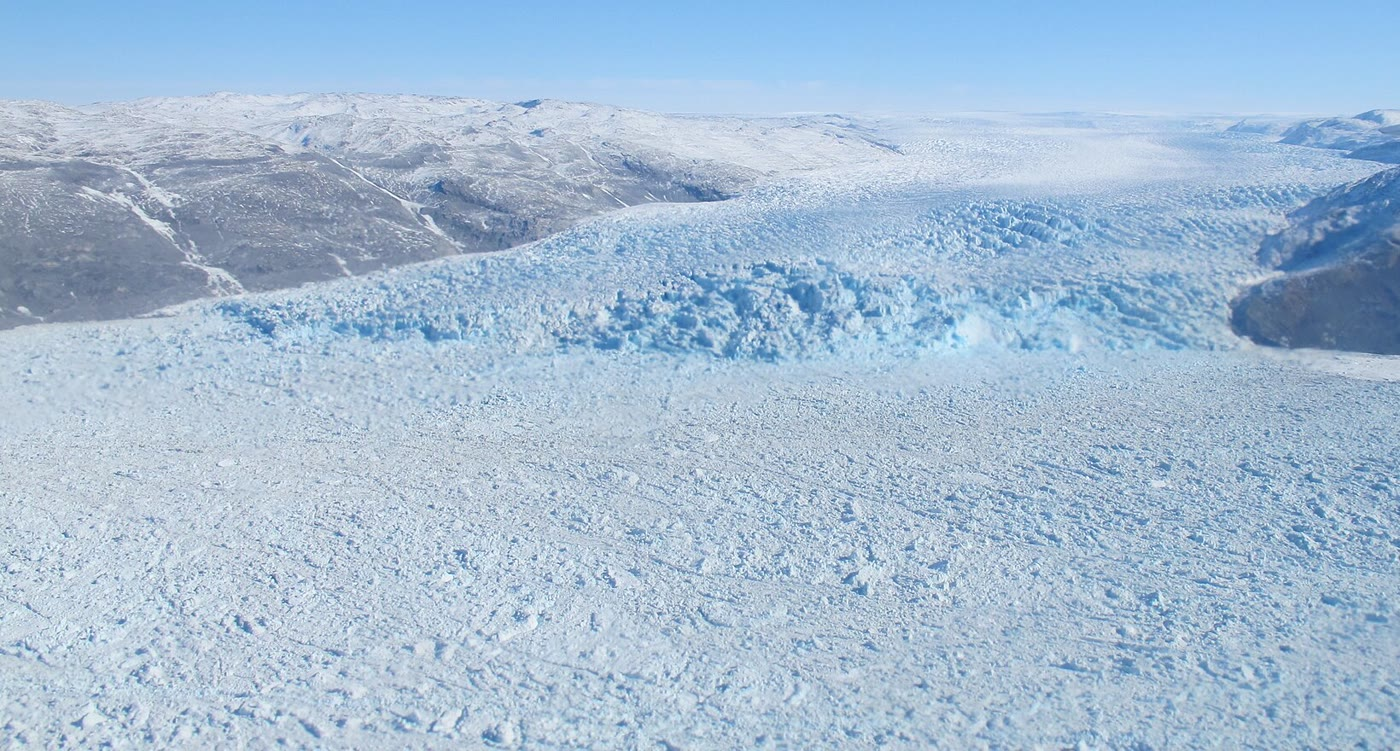
\includegraphics[width=0.82\linewidth]{images/book5/b3-greenland-outlet.jpg}

\par\smallskip{\small Uma geleira de descarga do manto de gelo da Groenlândia,
entre montanhas, terminando no mar em sua frente de desprendimento, a parede
partida de gelo azul que atravessa o centro da imagem; o fiorde à frente está
obstruído por gelo desprendido e gelo marinho. Fotografada de uma aeronave da
Operation IceBridge, da NASA, em abril de 2014 (NASA / Jim Yungel, domínio
público).}\label{fig:b3:glaciology:outlet}
\end{omfigure}
% ledger: photo:b3-greenland-outlet

\begin{inthefield}[Um acampamento sobre o gelo]
\begin{minipage}[t]{0.55\linewidth}\vspace{0pt}
Sobre um manto de gelo, os instrumentos dos glaciologistas se deslocam de trenó e vivem em
barracas. Para medir a velocidade com que o gelo se move, crava-se na neve um poste e
monta-se nele a antena de um receptor de navegação por satélite. Os receptores usados em
geodésia fixam uma posição com precisão de poucos centímetros; assim,
posições repetidas ao longo de semanas ou estações dão a velocidade e a direção do gelo, e a altura do poste,
medida de novo, dá o afinamento ou o espessamento
do gelo sob ele.
\end{minipage}\hfill
\begin{minipage}[t]{0.42\linewidth}\vspace{0pt}
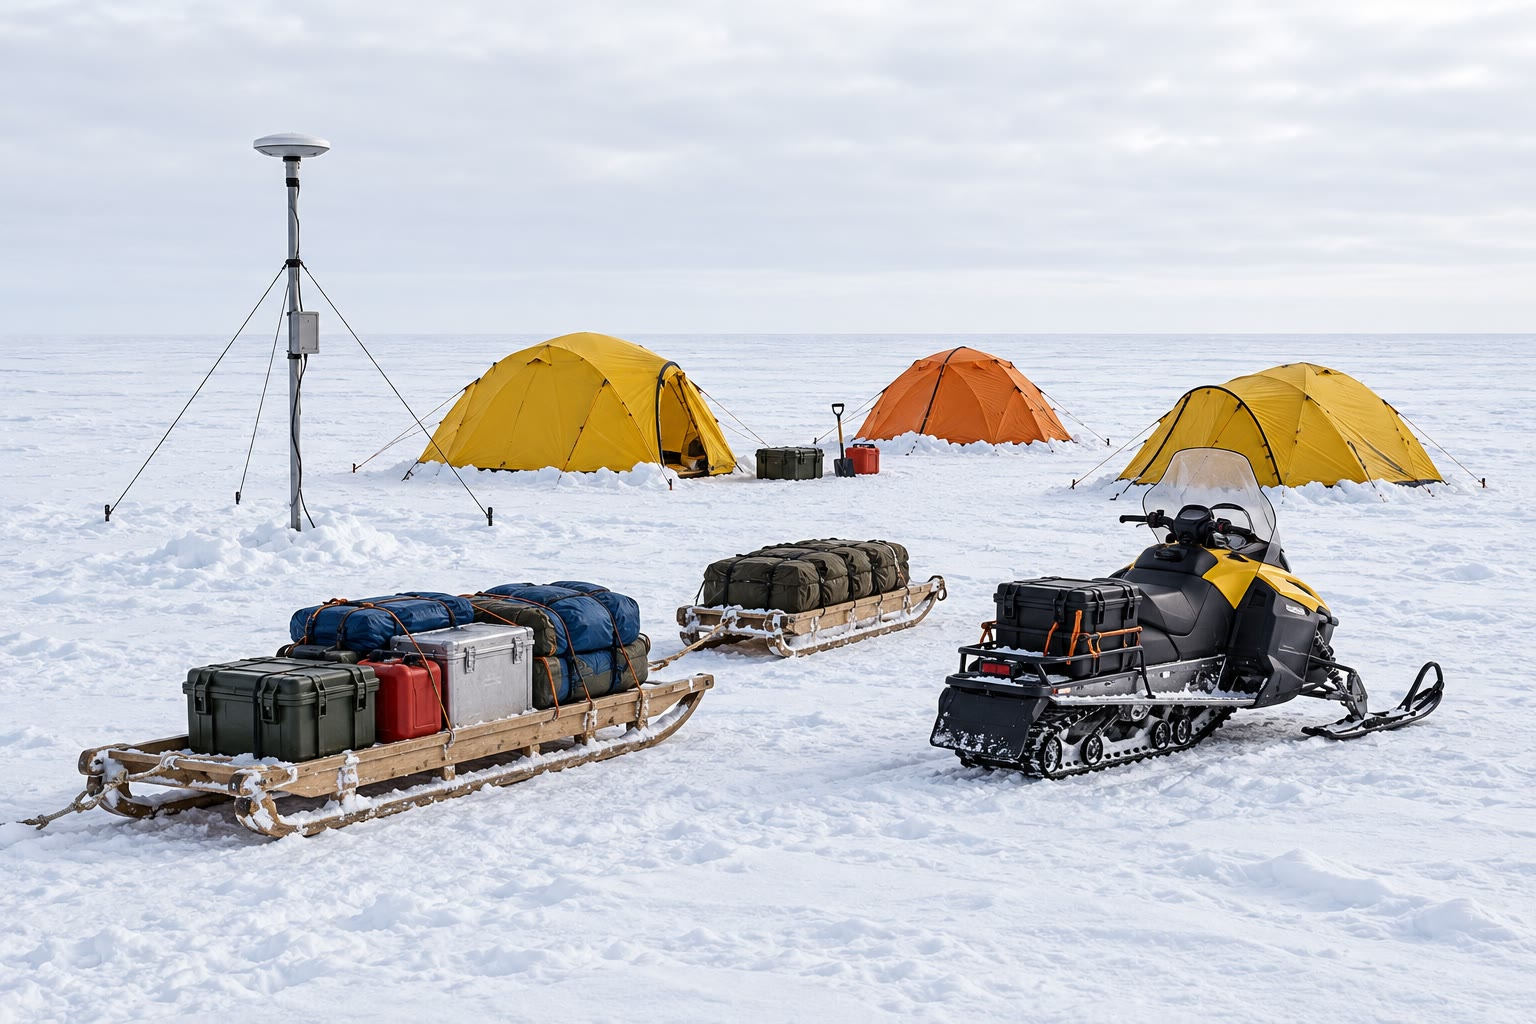
\includegraphics[width=\linewidth]{images/book5/ai/b3-glaciology-camp.jpg}

{\scriptsize Um acampamento de campo sobre um manto de gelo: barracas, trenós e uma
motoneve, e uma antena de navegação por satélite em um mastro sustentado por cabos
de tensão (Ilustração gerada por IA.)}
\end{minipage}
\end{inthefield}
% ledger: gps:high-end

\section{Gelo marinho e permafrost}\label{sec:b3:glaciology:sea-ice}

O gelo marinho se forma, cresce e derrete no oceano. No Ártico, ele atinge sua
maior área em março e sua menor em setembro.
% ledger: nsidc:sea-ice-def

\begin{definition}[Extensão do gelo marinho]\label{def:b3:glaciology:sea-ice}
A \emph{extensão do gelo marinho}\index{extensão do gelo marinho} é a área total das
células de um mapa de satélite em que o gelo marinho cobre mais de
\qty{15}{\percent} da superfície. Ela é maior que a área do gelo marinho,
que conta apenas o próprio gelo.
\end{definition}
% ledger: nsidc:sea-ice-def

Desde que os satélites passaram a mapeá-la, em 1979, a extensão do Ártico diminuiu, em março e bem mais em setembro,
à taxa de \qty{0.74}{\mega km^2} por década em
setembro, cerca de \qty{12}{\percent} da média de 1981--2010 por década, contra
\qty{0.38}{\mega km^2}, \qty{2.5}{\percent}, em março. A menor
extensão de setembro até agora, \qty{3.57}{\mega km^2}, ocorreu em 2012. O gelo marinho do Ártico
reflete \qtyrange{50}{70}{\percent} da luz solar, enquanto o oceano aberto reflete
cerca de \qty{6}{\percent}: ao perder o gelo, a superfície escurece, e isso é a
retroalimentação gelo--albedo do volume do segundo ano.
% ledger: data:b5-nsidc-extent, nsidc:sea-ice-reflect

O gelo marinho cresce na sua base, onde a água do mar congela sobre ele, e o calor latente
dessa congelação precisa ser conduzido para cima, através do gelo, até o ar frio.

\begin{theorem}[Lei de Stefan]\label{thm:b3:glaciology:stefan}
Um gelo marinho de condutividade térmica $k_i$, densidade $\rho_i$ e calor latente de
fusão $L$, com sua superfície mantida a uma temperatura $\Delta T$ abaixo do ponto de
congelamento da água subjacente, cresce, se o calor vindo do oceano for
desprezível, segundo
\[
h(t)^2 - h(0)^2 = \frac{2k_i\,\Delta T}{\rho_iL}\,t .
\]
Sob uma camada de neve de espessura $h_s$ e condutividade $k_s$, a taxa de
crescimento é $\mathrm dh/\mathrm dt = \Delta T/[\rho_iL(h/k_i + h_s/k_s)]$.
\end{theorem}

\begin{proof}
A temperatura no gelo fino é linear, do ponto de congelamento na
base até a temperatura da superfície no topo, de modo que o fluxo de calor através dele é
$k_i\Delta T/h$ ou, através do gelo e da neve em série, $\Delta T/(h/k_i +
h_s/k_s)$. A congelação de uma camada $\mathrm dh$ libera $\rho_iL\,\mathrm dh$ por
unidade de área, que esse fluxo precisa remover: $\rho_iL\,\mathrm dh/\mathrm dt
= k_i\Delta T/h$. Então $\mathrm d(h^2)/\mathrm dt = 2k_i\Delta T/(\rho_iL)$.
\end{proof}

Com $k_i = \qty{2.03}{W.m^{-1}.K^{-1}}$, $L = \qty{3.34e5}{J/kg}$ e
$\rho_i = \qty{917}{kg/m^3}$, uma superfície \qty{20}{K} abaixo do congelamento cresce
\qty{1.5}{m} de gelo em cem dias e \qty{2.1}{m} em duzentos.
A neve, com condutividade de \qty{0.30}{W.m^{-1}.K^{-1}}, é um bom
isolante: \qty{20}{cm} dela já reduzem o crescimento em mais da metade. Gelo espesso cresce
devagar, gelo fino cresce depressa: a lei tende a uniformizar a espessura do gelo
após um verão de degelo.
% ledger: cice:constants, iapws:ice-density

\begin{omfigure}
\begin{tikzpicture}
\begin{groupplot}[group style={group size=2 by 1, horizontal sep=1.5cm},
  width=0.48\linewidth, height=0.4\linewidth,
  tick label style={font=\scriptsize}, label style={font=\small}, title style={font=\small}]
\nextgroupplot[xlabel={ano}, ylabel={extensão (\unit{\mega km^2})}, xmin=1977, xmax=2028,
  ymin=0, ymax=18, title={Extensão do gelo marinho do Ártico},
  xticklabel style={/pgf/number format/1000 sep={}},
  legend style={font=\scriptsize, at={(0.03,0.66)}, anchor=west}]
% computed in figdata/bachelor-3/sea_ice.py
\addplot[omDef, thick, mark=*, mark size=0.9pt] table[x=year, y=mar] {figdata/out/bachelor-3-sea_ice-extent.dat};
\addlegendentry{março}
\addplot[omThm, thick, mark=*, mark size=0.9pt] table[x=year, y=sep] {figdata/out/bachelor-3-sea_ice-extent.dat};
\addlegendentry{setembro}
\addplot[black!60, densely dashed, forget plot] table[x=year, y=mar] {figdata/out/bachelor-3-sea_ice-trend.dat};
\addplot[black!60, densely dashed, forget plot] table[x=year, y=sep] {figdata/out/bachelor-3-sea_ice-trend.dat};
\nextgroupplot[xlabel={dias de congelamento}, ylabel={espessura do gelo (\unit{m})}, xmin=0, xmax=200,
  ymin=0, ymax=2.4, title={crescimento, $\Delta T = \qty{20}{K}$},
  legend style={font=\scriptsize, at={(0.97,0.03)}, anchor=south east}]
\addplot[omMeth, thick] table[x=day, y=h0] {figdata/out/bachelor-3-sea_ice-stefan.dat};
\addlegendentry{gelo nu}
\addplot[omDef, thick, densely dashed] table[x=day, y=hs] {figdata/out/bachelor-3-sea_ice-stefan.dat};
\addlegendentry{sob \qty{20}{cm} de neve}
\end{groupplot}
\end{tikzpicture}

\par\smallskip{\small À esquerda, a \omterm{def:b3:glaciology:sea-ice}{extensão média do gelo marinho} do Ártico em março e em
setembro, de 1979 a 2026 (NSIDC Sea Ice Index, versão~4), com tendências por mínimos
quadrados (tracejadas): \qty{-0.38}{\mega km^2} e \qty{-0.74}{\mega km^2} por
década. À direita, o crescimento do gelo marinho por condução sob uma superfície
\qty{20}{K} abaixo do congelamento, sem calor do oceano: gelo nu, pela lei de Stefan,
e o mesmo gelo sob \qty{20}{cm} de neve.}\label{fig:b3:glaciology:sea-ice}
\end{omfigure}
% ledger: data:b5-nsidc-extent, cice:constants

Permafrost é o solo que se mantém a \qty{0}{\celsius} ou abaixo disso por dois anos
ou mais. Ele se encontra sob cerca de um quarto da terra emersa do
Hemisfério Norte.
% ledger: nsidc:permafrost

\begin{definition}[Camada ativa]\label{def:b3:glaciology:permafrost}
A \emph{camada ativa}\index{camada ativa} é a camada de solo acima do permafrost que degela
a cada verão e volta a congelar a cada inverno.
\end{definition}

Sua espessura é determinada, como o crescimento do gelo marinho, pela condução de calor
para dentro do solo durante a estação de degelo, em oposição ao calor latente do
gelo do solo. As temperaturas do permafrost aumentaram nas últimas três a
quatro décadas em todas as regiões de permafrost (alta confiança);
o permafrost se aqueceu globalmente em \qty{0.29}{\celsius} [\numrange{0.17}{0.41}]
entre 2007 e 2016 (confiança média), e um aumento da espessura da \omterm{def:b3:glaciology:permafrost}{camada
ativa} é um fenômeno pan-ártico (confiança média).
Onde o gelo derrete, o solo pode colapsar.
% ledger: ar6ch9:permafrost, nsidc:permafrost-thaw

\section{A criosfera e o nível do mar}\label{sec:b3:glaciology:sea-level}

O balanço do nível do mar do volume do segundo ano soma a expansão do oceano em aquecimento
à água acrescentada pelo gelo e pela terra. Dos
\qty{3.69}{mm/yr} de elevação do nível do mar observados em 2006--2018, as geleiras
contribuíram com \qty{0.62}{mm/yr}, a Groenlândia com \qty{0.63}{mm/yr} e a Antártida
com \qty{0.37}{mm/yr}: o gelo, em conjunto, superou a expansão do oceano,
\qty{1.39}{mm/yr}.
% ledger: ar6ch9:table95

\begin{dated}{2021}
A Groenlândia perdeu \qty{4890}{Gt} de gelo entre 1992 e 2020 [4140 a 5640],
\qty{13.5}{mm} de nível do mar, com taxas que subiram de \qty{39}{Gt/yr} na
década de 1990 para \qty{243}{Gt/yr} em 2010--2019, por vazão e, cada vez mais,
por degelo superficial (alta confiança). A Antártida perdeu \qty{2670}{Gt}
[1800 a 3540], \qty{7.4}{mm}, com taxa que subiu de \qty{49}{Gt/yr} na
década de 1990 para \qty{148}{Gt/yr} em 2010--2019; as perdas vieram das geleiras de saída da
Antártida Ocidental, sobretudo pelo derretimento das plataformas de gelo pela base (alta
confiança). As geleiras fora dos mantos de gelo perderam \qty{6200}{Gt}
entre 1993 e 2019, \qty{17.1}{mm}, mais em 2010--2019 do que em qualquer outra década
do registro (confiança muito alta). A Groenlândia continuará a perder massa
ao longo deste século em todos os cenários considerados (praticamente
certo), e o mesmo ocorrerá com a Antártida (provável): até 2100, a Groenlândia provavelmente acrescenta
\qtyrange{0.01}{0.10}{m} ao nível do mar sob um cenário de baixas emissões
e \qtyrange{0.09}{0.18}{m} sob um de emissões muito altas; a Antártida,
\qtyrange{0.03}{0.27}{m} e \qtyrange{0.03}{0.34}{m}. O oceano Ártico
provavelmente ficará praticamente livre de gelo marinho, com menos de
\qty{1}{\mega km^2} dele, em seu mínimo de setembro, pela primeira vez
antes de 2050 em todos os cenários considerados.
\end{dated}
% ledger: ar6ch9:greenland, ar6ch9:antarctica, ar6ch9:glaciers, ar6ch9:ice-sheet-proj, ar6ch9:sea-ice

As perdas das capas de gelo são as do Capítulo~\ref{ch:b3:gravity-geodesy},
medidas por altimetria, por gravimetria e pela diferença entre a neve
que cai e o gelo que escoa para fora: três métodos independentes reunidos
em uma única estimativa.
% ledger: data:b5-imbie

\section{Exercícios}

\begin{exercise}[$\star$]\label{exo:b3:glaciology:1}
Uma geleira de vale com \qty{250}{m} de espessura escoa por uma encosta de \ang{3}. Calcule
a tensão de cisalhamento basal e compare-a com as tensões basais de
geleiras reais, da ordem de um bar.
\end{exercise}

\begin{exercise}[$\star$]\label{exo:b3:glaciology:2}
(a)~O manto de gelo da Groenlândia contém cerca de \qty{2.9}{\mega km^3} de gelo de
densidade \qty{917}{kg/m^3}. Calcule sua massa e seu \omterm{def:b3:glaciology:sle}{equivalente em nível do mar} em
\qty{360}{Gt/mm}, e compare com os \qty{7.4}{m} normalmente citados.
(b)~Faça o mesmo para a Antártida, com \qty{30}{\mega km^3}, citada como cerca de
\qty{58}{m}. Por que os dois valores se comparam de forma tão diferente?
\end{exercise}
% ledger: nsidc:ice-sheets

\begin{exercise}[$\star$]\label{exo:b3:glaciology:3}
Uma geleira tem uma \omterm{def:b3:glaciology:mass-balance}{zona de acumulação} de \qty{6}{km^2} com balanço médio de
\qty{+1.2}{m} de equivalente em água, e uma \omterm{def:b3:glaciology:mass-balance}{zona de ablação} de \qty{4}{km^2} com
\qty{-2.1}{m}. Calcule seu balanço líquido em metros cúbicos de água, seu balanço
específico médio e sua razão de área de acumulação. Ela está crescendo ou
diminuindo?
\end{exercise}

\begin{exercise}[$\star$]\label{exo:b3:glaciology:4}
No \omterm{def:b3:glaciology:firn}{fechamento dos poros}, o \omterm{def:b3:glaciology:firn}{firn} tem densidade de \qtyrange{820}{830}{kg/m^3}.
Qual fração de seu volume ainda é espaço poroso (gelo:
\qty{917}{kg/m^3})?
\end{exercise}
% ledger: firn:close-off

\begin{exercise}[$\star\star$]\label{exo:b3:glaciology:5}
Uma geleira temperada (gelo a \qty{0}{\celsius}, $A =
\qty{1.4e-16}{Pa^{-3}.yr^{-1}}$) tem \qty{300}{m} de espessura em uma encosta de
\ang{3}. Calcule sua velocidade superficial apenas por deformação interna. Por qual
fator a velocidade mudaria se ela fosse duas vezes mais espessa? E se a encosta fosse
reduzida à metade?
\end{exercise}

\begin{exercise}[$\star\star$]\label{exo:b3:glaciology:6}
A partir das constantes de Paterson--Budd, calcule o \omterm{def:b3:glaciology:glen}{fator de taxa} a
\qty{-25}{\celsius} e a \qty{-10}{\celsius}, e a razão entre as velocidades de
duas massas de gelo idênticas a \qty{0}{\celsius} e a \qty{-25}{\celsius}.
\end{exercise}
% ledger: pism:rheology, codata:R

\begin{exercise}[$\star\star$]\label{exo:b3:glaciology:7}
Calcule a maior espessura de um manto de gelo plástico com \qty{1000}{km} do centro
até a margem, com $\tau_0 = \qty{100}{kPa}$, e compare com a
maior espessura do gelo antártico, quase \qty{4.9}{km}.
\end{exercise}
% ledger: nsidc:ice-sheets

\begin{exercise}[$\star\star$]\label{exo:b3:glaciology:8}
Uma geleira com \qty{200}{m} de espessura perde \qty{5}{m} de gelo por ano em sua língua.
Estime seu tempo de resposta. Se o clima aquecesse abruptamente e depois
permanecesse constante, por quanto tempo seu comprimento continuaria a variar?
\end{exercise}

\begin{exercise}[$\star\star$]\label{exo:b3:glaciology:9}
(a)~Usando a lei de Stefan com $\Delta T = \qty{20}{K}$, calcule a espessura
do gelo marinho sem cobertura após 100 dias, e o tempo necessário para atingir \qty{3}{m}.
(b)~O que isso sugere sobre gelo com mais de \qty{3}{m} de espessura?
\end{exercise}
% ledger: cice:constants

\begin{exercise}[$\star\star\star$]\label{exo:b3:glaciology:10}
(a)~Onde o leito está \qty{800}{m} abaixo do nível do mar, qual é a espessura do gelo na
\omterm{def:b3:glaciology:grounding-line}{linha de encalhe}? (b)~Usando o fluxo da laje $q \propto H^{n+2}$ para uma dada
inclinação da superfície, por qual fator o fluxo do gelo apoiado aumenta se a
\omterm{def:b3:glaciology:grounding-line}{linha de encalhe} recuar até onde o leito está a \qty{900}{m} de profundidade? (c)~Explique
por que um leito que se aprofunda para o interior torna o recuo autorreforçado, e o que
uma plataforma de gelo altera.
\end{exercise}
% ledger: iapws:ice-density, noaa:seawater-1025

\begin{exercise}[$\star\star\star$]\label{exo:b3:glaciology:11}
Mostre que o volume de uma capa de gelo plástica circular de raio $R$ é $V =
\frac{8\pi}{15}\sqrt{2\tau_0/(\rho g)}\,R^{5/2}$. Por qual fator seu \omterm{def:b3:glaciology:sle}{equivalente em nível do mar}
cresce se o raio dobrar?
\end{exercise}

\begin{exercise}[$\star\star\star$]\label{exo:b3:glaciology:12}
A extensão média do Ártico foi de \qty{16.34}{\mega km^2} em março de 1979 e de
\qty{14.13}{\mega km^2} em março de 2026; em setembro, \num{7.05} e
\qty{4.81}{\mega km^2}. (a)~Calcule a variação relativa em cada mês.
(b)~Dê duas razões físicas pelas quais a extensão de setembro caiu muito
mais rapidamente do que a extensão de março.
\end{exercise}
% ledger: data:b5-nsidc-extent

\section{Problema: A Capa de Gelo de Arkel}

\begin{problem}[{Problema de fim de semana --- a forma, o fluxo, o balanço e o
equivalente em nível do mar de uma capa de gelo inventada}]
\label{pb:b3:glaciology:1}
A capa de gelo inventada de Arkel repousa sobre um platô plano. Ela é quase
circular, com \qty{20}{km} de raio, e seu gelo está a cerca de \qty{-10}{\celsius}. Tome
$\rho = \qty{917}{kg/m^3}$ e $g = \qty{9.81}{m/s^2}$.

\medskip\noindent\textbf{Parte I --- A capa é plástica?}
\begin{enumerate}
\item Mostre que, sob gelo de espessura $H$ com uma pequena inclinação
  superficial $\alpha$, a tensão de cisalhamento basal é de cerca de $\rho gH\alpha$.
\item Sondagens de radar e levantamentos a \qty{5}, \qty{10} e \qty{15}{km} do centro
  fornecem espessuras de 580, 470 e \qty{335}{m} e inclinações superficiais de
  \num{0.0190}, \num{0.0240} e \num{0.0330}. Calcule a tensão de cisalhamento basal
  nos três pontos.
\item A capa está próxima de ser plástica? Qual tensão de escoamento você adota?
\item Com $\tau_0 = \qty{100}{kPa}$, calcule $2\tau_0/(\rho g)$.
\item Preveja a espessura nos três pontos a partir do perfil plástico e compare
  com as sondagens.
\end{enumerate}

\medskip\noindent\textbf{Parte II --- Forma e volume.}
\begin{enumerate}[resume]
\item Calcule a espessura no centro.
\item Mostre que o volume é $V = \frac{8\pi}{15}\sqrt{2\tau_0/(\rho
  g)}\,R^{5/2}$.
\item Calcule o volume em quilômetros cúbicos.
\item Calcule a área e a espessura média.
\item Uma capa de gelo duas vezes mais larga sobre o mesmo platô: por qual fator o seu
  volume é maior?
\end{enumerate}

\medskip\noindent\textbf{Parte III --- Escoamento e balanço.}
\begin{enumerate}[resume]
\item Calcule o \omterm{def:b3:glaciology:glen}{fator de taxa} a \qty{-10}{\celsius} em
  \unit{Pa^{-3}.yr^{-1}}.
\item A \qty{10}{km} do centro, tratando o gelo como uma laje, calcule
  a velocidade superficial por deformação interna.
\item Calcule o fluxo de gelo por unidade de largura ali e a velocidade média da
  coluna.
\item Em estado estacionário, o fluxo que sai do círculo de raio
  \qty{10}{km} é igual ao balanço ganho em seu interior. Qual balanço médio, em
  metros de gelo por ano, isso exige?
\item A linha de equilíbrio situa-se \qty{450}{m} acima do platô. Onde ela está
  na capa, e qual é a razão da área de acumulação?
\item Se o gelo se aquecesse até \qty{0}{\celsius}, por qual fator as
  velocidades aumentariam? O que aconteceria com a forma da capa?
\end{enumerate}

\medskip\noindent\textbf{Parte IV --- Nível do mar.}
\begin{enumerate}[resume]
\item Calcule a massa da capa em gigatoneladas.
\item Calcule o seu \omterm{def:b3:glaciology:sle}{equivalente em nível do mar} em milímetros.
\item Se a capa inteira afinasse \qty{0.5}{m} de gelo por ano, sem
  escoar, quanto tempo ela duraria?
\item Por que a capa real desapareceria antes disso, assim que começasse a
  afinar?
\item Na taxa em que a Groenlândia perdeu gelo em 2010--2019, quanto tempo levaria
  para perder uma massa igual à da capa Arkel?
\item Forneça o \omterm{def:b3:glaciology:sle}{equivalente em nível do mar} da capa de gelo Arkel, em milímetros,
  com uma casa decimal.
\end{enumerate}
\end{problem}
% ledger: pism:rheology, data:b5-imbie, ar6ch9:greenland, ar6ch9:faq91
